%%%%%%%%%%%%%%%%%%%%%%%%%%%%%%%%%%%%%%%%%
% University Assignment Title Page 
% LaTeX Template
% Version 1.0 (27/12/12)
%
% This template has been downloaded from:
% http://www.LaTeXTemplates.com
%
% Original author:
% WikiBooks (http://en.wikibooks.org/wiki/LaTeX/Title_Creation)
%
% License:
% CC BY-NC-SA 3.0 (http://creativecommons.org/licenses/by-nc-sa/3.0/)
% 
% Instructions for using this template:
% This title page is capable of being compiled as is. This is not useful for 
% including it in another document. To do this, you have two options: 
%
% 1) Copy/paste everything between \begin{document} and \end{document} 
% starting at \begin{titlepage} and paste this into another LaTeX file where you 
% want your title page.
% OR
% 2) Remove everything outside the \begin{titlepage} and \end{titlepage} and 
% move this file to the same directory as the LaTeX file you wish to add it to. 
% Then add \input{./title_page_1.tex} to your LaTeX file where you want your
% title page.
%
%%%%%%%%%%%%%%%%%%%%%%%%%%%%%%%%%%%%%%%%%

%----------------------------------------------------------------------------------------
%	PACKAGES AND OTHER DOCUMENT CONFIGURATIONS
%----------------------------------------------------------------------------------------

\documentclass[12pt]{article}
\usepackage[utf8]{inputenc}
\usepackage[T1]{fontenc}
\usepackage{url}
\def\UrlBreaks{\do\/\do-}
\usepackage{fixltx2e}
\usepackage{graphicx}
\usepackage{xcolor}
\usepackage{caption}
\usepackage{float}
\usepackage{wrapfig}
\usepackage{amssymb}
\usepackage[colorinlistoftodos,prependcaption,textsize=tiny]{todonotes}
\usepackage{soul}
\usepackage{textcomp}
\usepackage{marvosym}
\usepackage[integrals]{wasysym}
\usepackage{latexsym}
\usepackage{amssymb}
\usepackage{hyperref}
\tolerance=1000
\usepackage{amsmath}
\usepackage{hyperref}
\usepackage{setspace}
\onehalfspacing
\usepackage[raggedright,bf,sf]{titlesec}
\usepackage{fullpage}
\usepackage{xcolor}
\usepackage{listings}

\begin{document}
\begin{titlepage}


\newcommand{\HRule}{\rule{\linewidth}{0.5mm}} % Defines a new command for the horizontal lines, change thickness here

\center % Center everything on the page
 
%----------------------------------------------------------------------------------------
%	HEADING SECTIONS
%----------------------------------------------------------------------------------------

\textsc{\Large DAT250}\\[0.5cm] % Major heading such as course name
\textsc{\large Advanced Software Technologies}\\[0.5cm] % Minor heading such as course title

%----------------------------------------------------------------------------------------
%	TITLE SECTION
%----------------------------------------------------------------------------------------

\HRule \\[0.4cm]
{ \huge \bfseries Assignment 1}\\[0.4cm] % Title of your document
\HRule \\[1.5cm]
 
%----------------------------------------------------------------------------------------
%	AUTHOR SECTION
%----------------------------------------------------------------------------------------

% If you don't want a supervisor, uncomment the two lines below and remove the section above
\Large \emph{Author:}\\
Jostein Kringlen, Kristian Rosland, \\André Dyrstad, Didrik Sæther\\[3cm] % Your name

%----------------------------------------------------------------------------------------
%	DATE SECTION
%----------------------------------------------------------------------------------------

{\large https://github.com/Diddern/DAT250-auction}\\[3cm]
{\large \today}\\[3cm] % Date, change the \today to a set date if you want to be precise

%----------------------------------------------------------------------------------------
%	LOGO SECTION
%----------------------------------------------------------------------------------------

%\includegraphics{Logo}\\[1cm] % Include a department/university logo - this will require the graphicx package
 
%----------------------------------------------------------------------------------------

\vfill % Fill the rest of the page with whitespace

\end{titlepage}

% Write text here.

\section{Use Case Diagram}

\begin{figure}[H]
  \caption{Use Case Diagram}
  \centering
    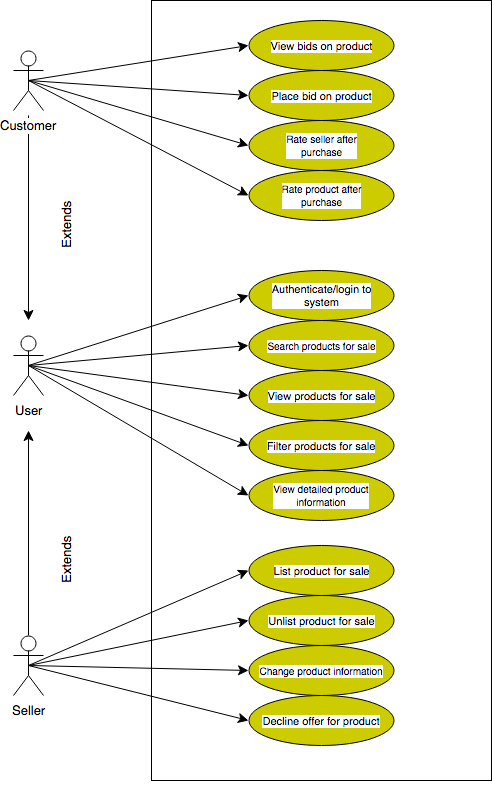
\includegraphics[scale=0.7]{figures/Use-Case}
\end{figure}

\section{Domain model}

\begin{figure}[H]
  \caption{Domain model}
  \centering
    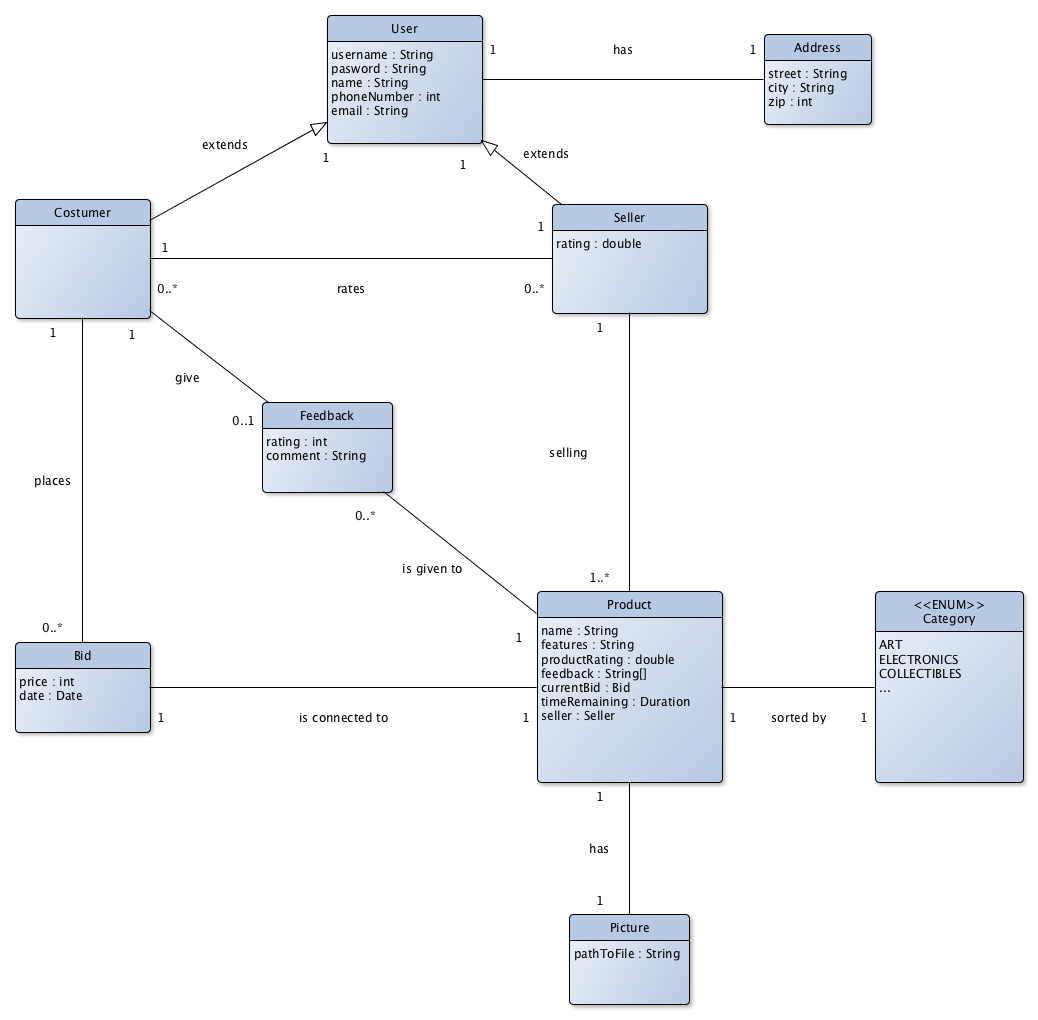
\includegraphics[scale=0.38]{figures/domain-diagram.png}
\end{figure}

\section{Application Flow Diagram}

\begin{figure}[H]
    \caption{Application Flow Diagram}
    \centering
    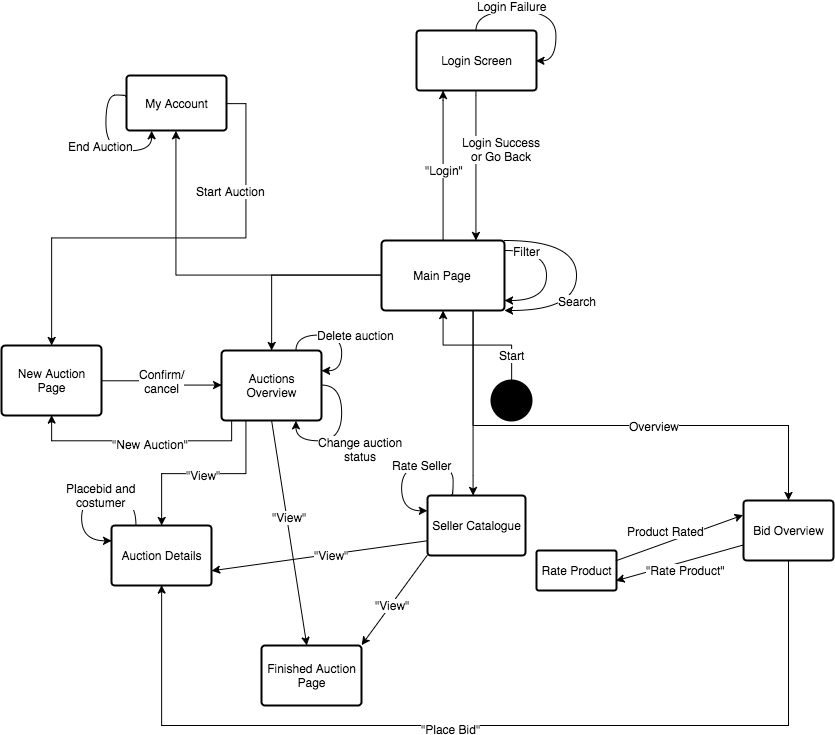
\includegraphics[scale=0.5]{figures/flowchart.png}
\end{figure}


\section{User Screens	}
\begin{figure}[H]
  \caption{Login-page}
  \centering
    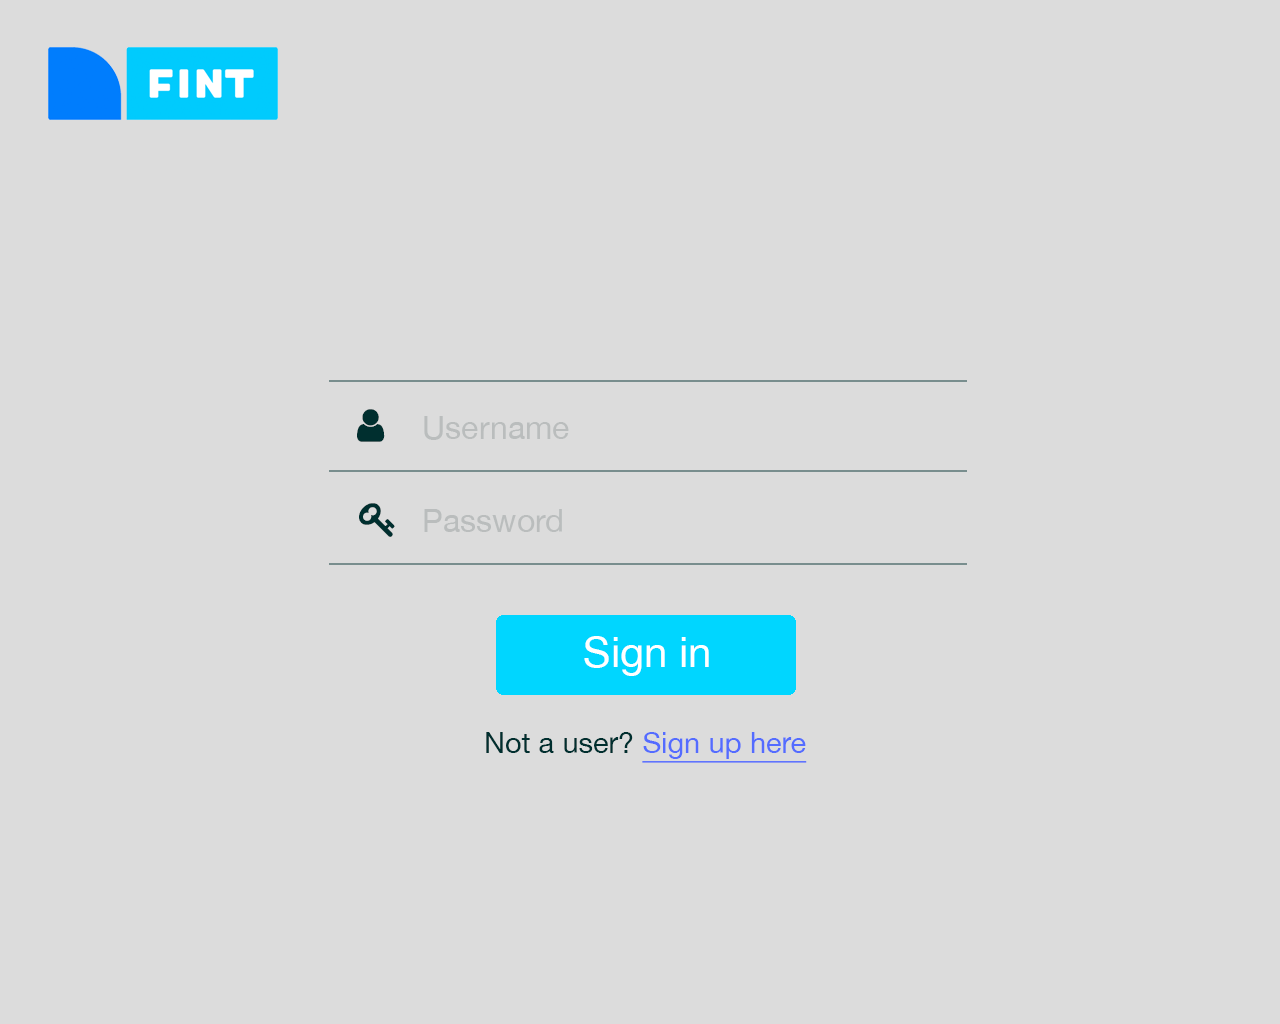
\includegraphics[scale=0.38]{figures/Login}
\end{figure}

\begin{figure}[H]
  \caption{Frontpage without login}
  \centering
    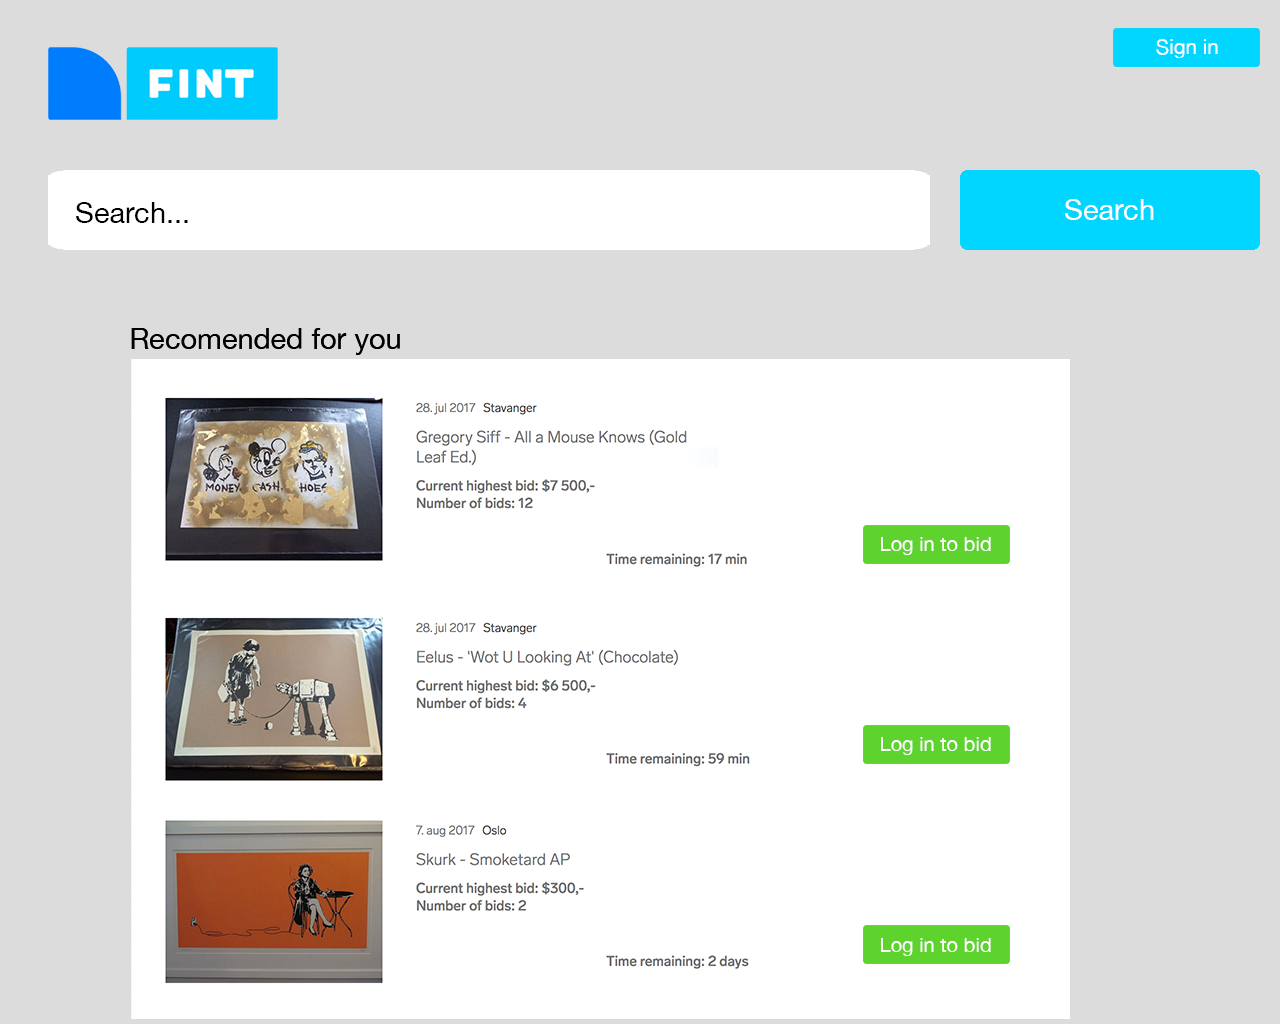
\includegraphics[scale=0.38]{figures/Frontpage}
\end{figure}

\begin{figure}
	\caption{Frontpage after login}
	\centering
		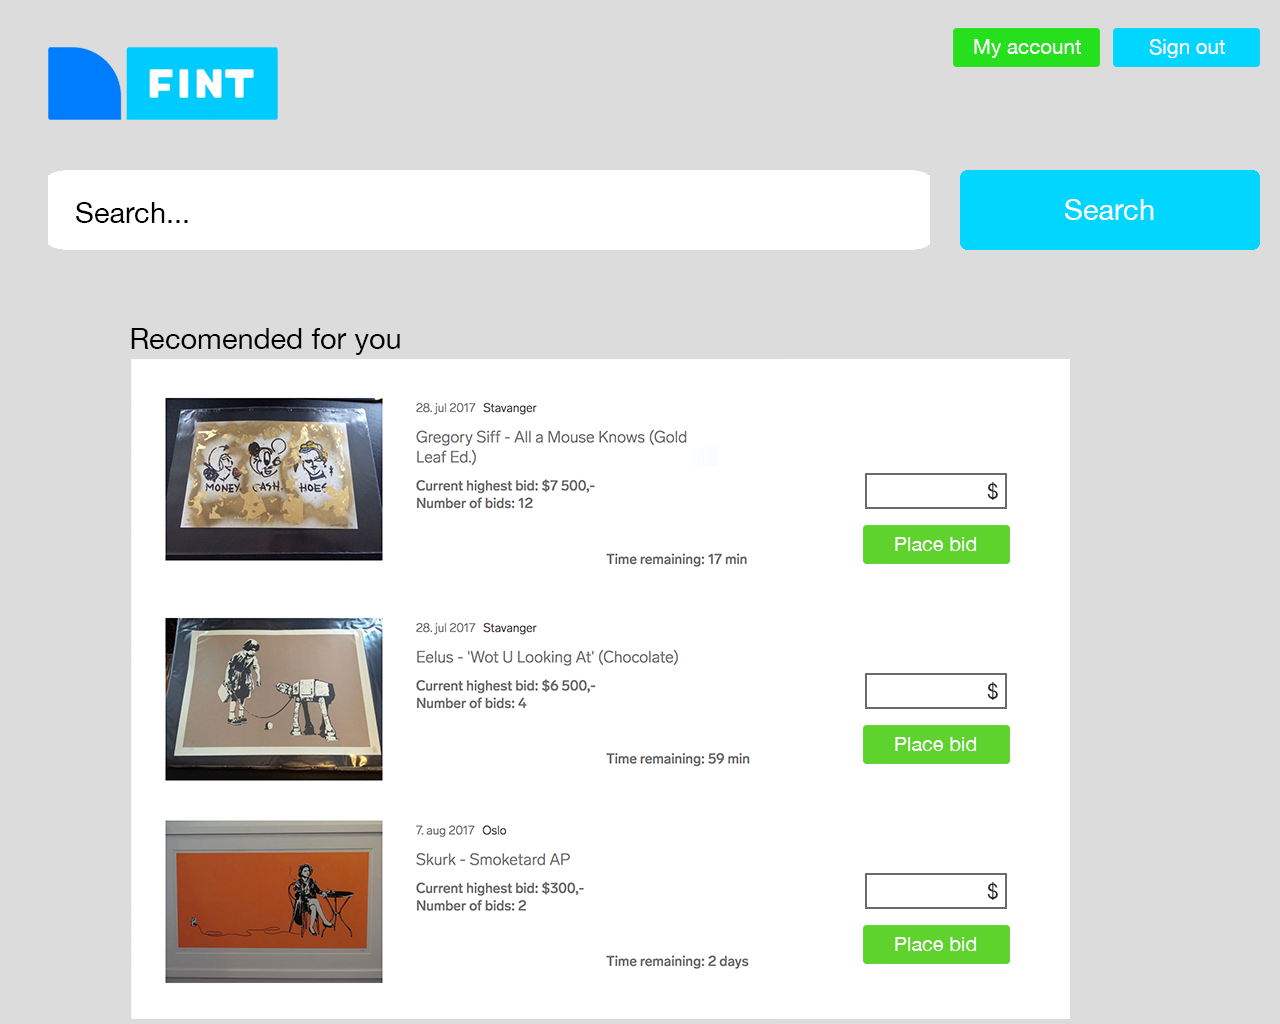
\includegraphics[scale=0.38]{figures/Frontpage-after-login}
\end{figure}

\begin{figure}
	\caption{My account}
	\centering
		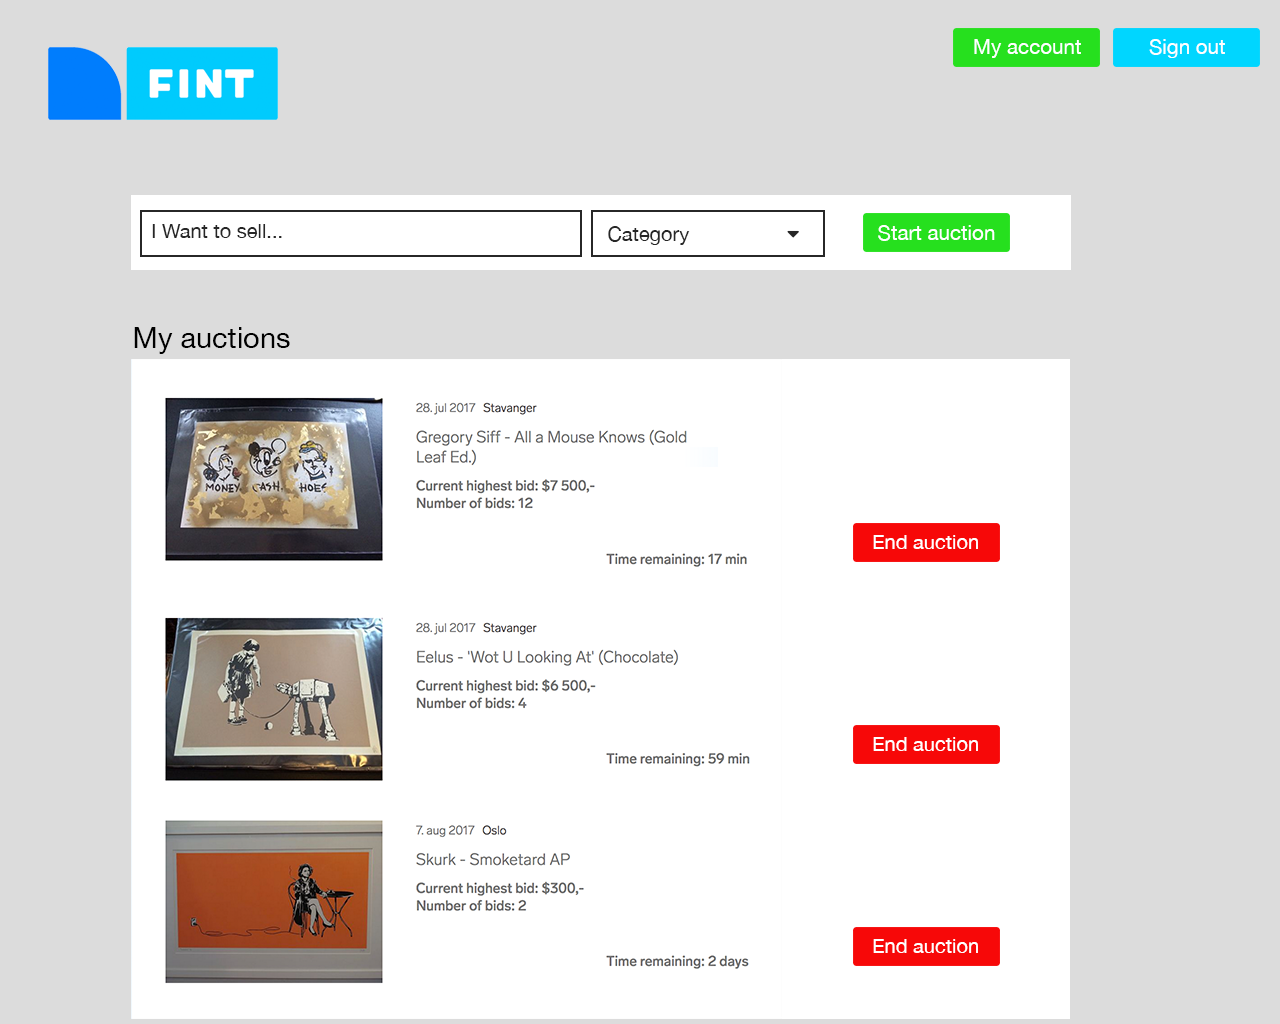
\includegraphics[scale=0.38]{figures/my-account}
\end{figure}

\begin{figure}
	\caption{Detailed view of product}
	\centering
		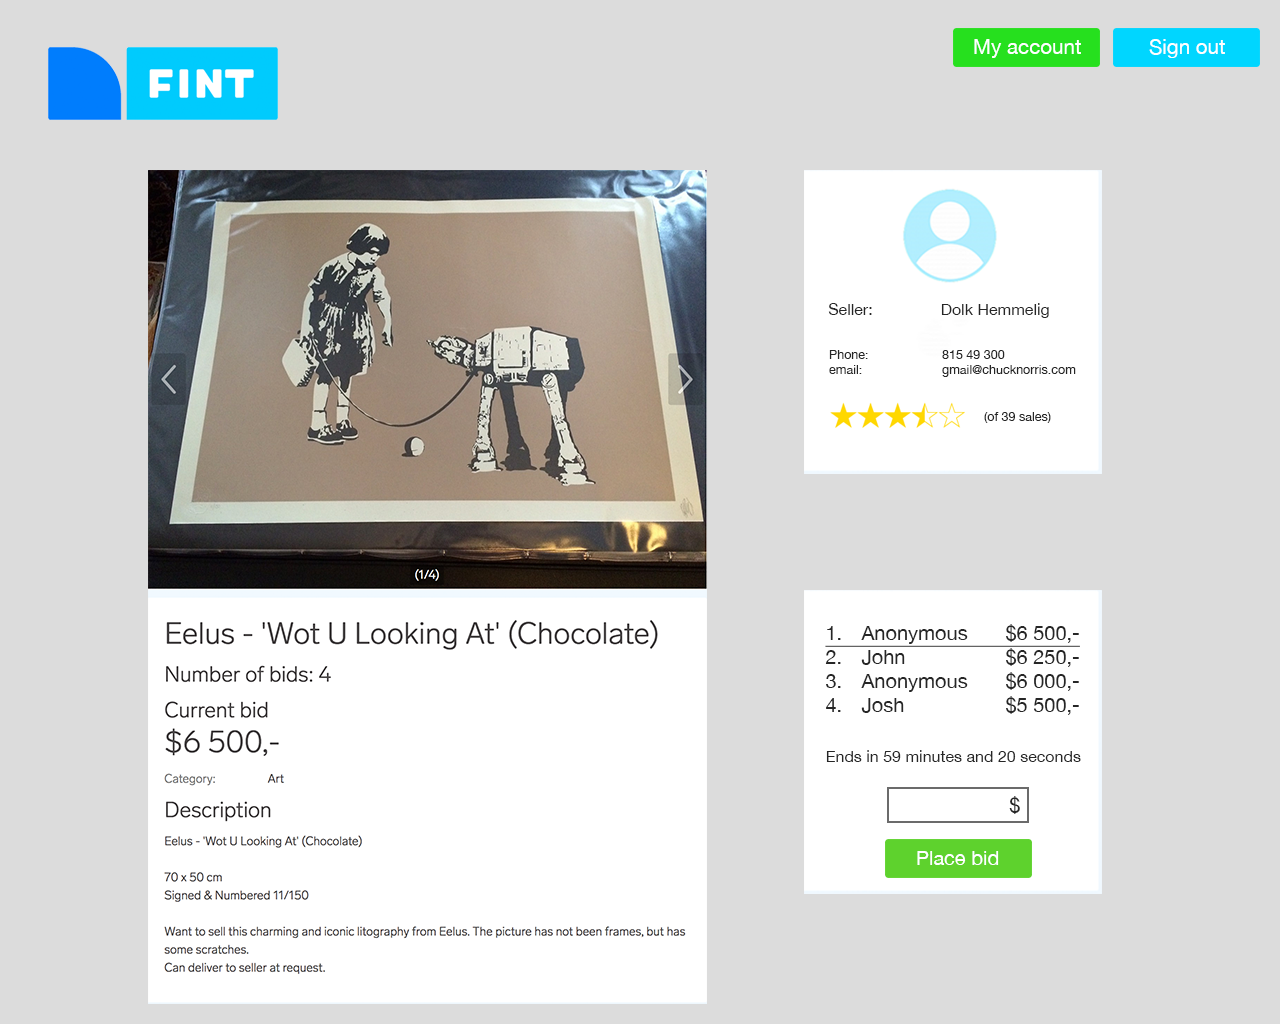
\includegraphics[scale=0.38]{figures/detailed-view-of-product}
\end{figure}

\begin{figure}
	\caption{Detailed view of product after finished auction}
	\centering
		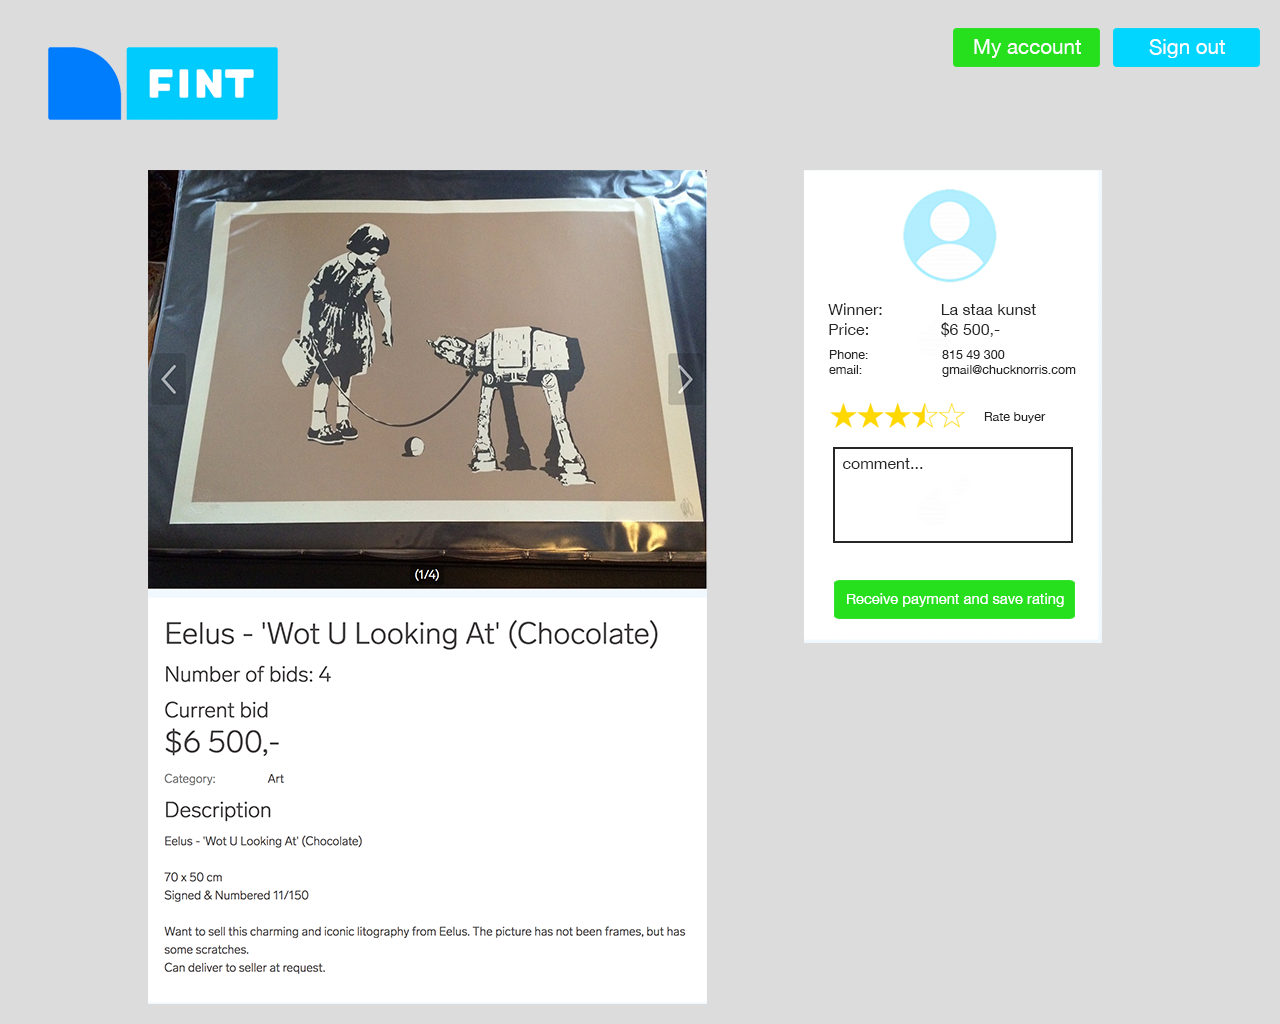
\includegraphics[scale=0.38]{figures/detailed-view-finished-aucution}
\end{figure}

\begin{figure}
	\caption{Create new auction}
	\centering
		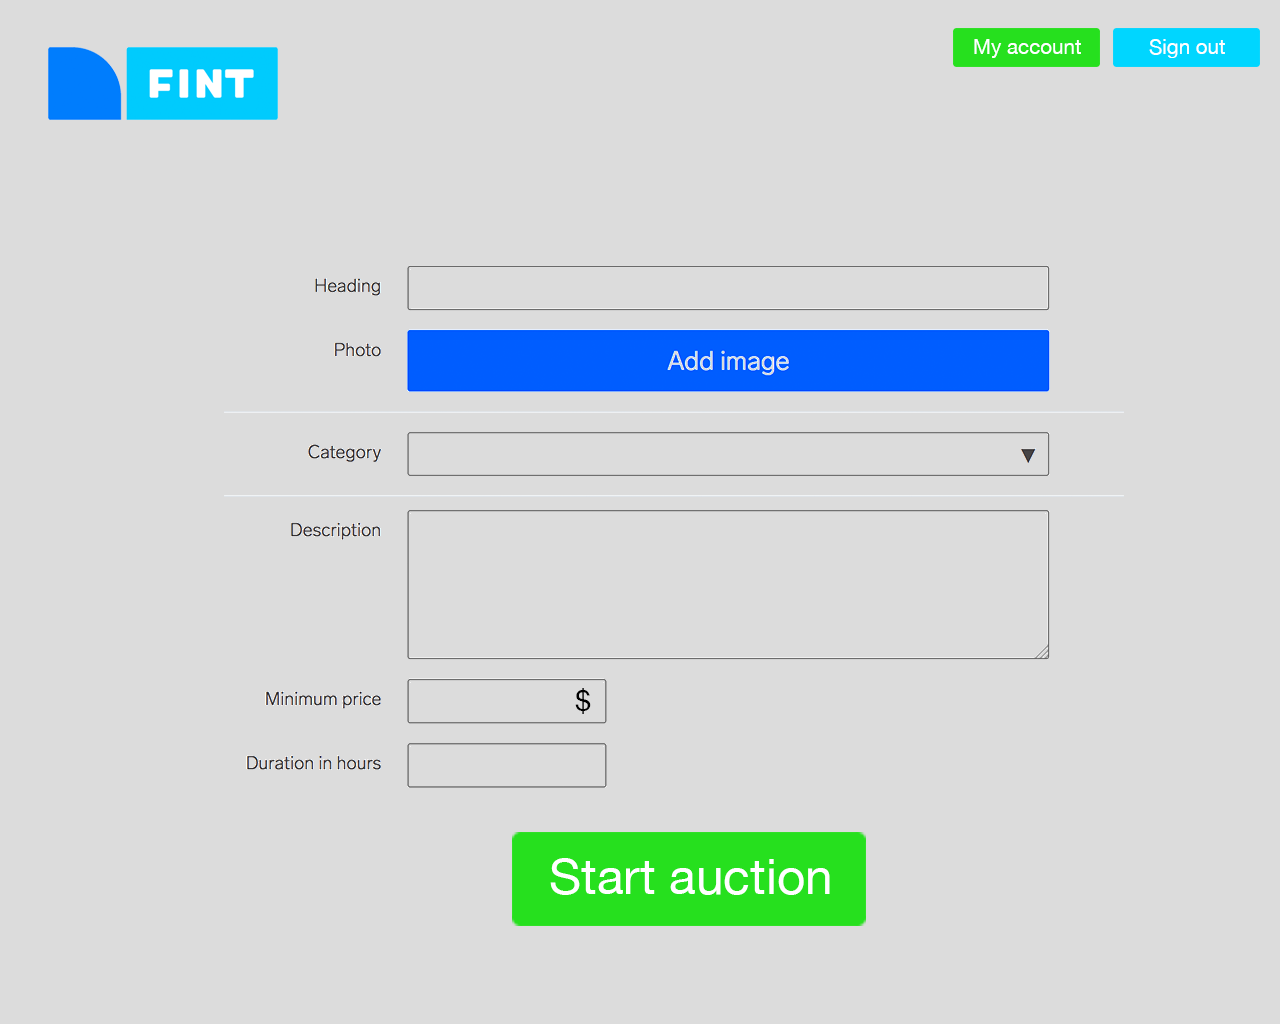
\includegraphics[scale=0.38]{figures/Create-new-auction}
\end{figure}


\end{document}
